\documentclass[10pt]{yerbaformat}
\title{数学物理方程 Notes\footnote{EEEEEErin~}}
\date{\today}

\begin{document}
\author{}
\maketitle
\tableofcontents
\footnotesize

\section{\href{https://wenku.baidu.com/view/cf58eb62ed630b1c58eeb506.html}{波动方程}}

\subsection{达朗贝尔公式和波的传播}

\par 端点值初始条件和初始时刻状态初始条件合称为定解条件. 方程对各阶导数线性称为线性方程, 对于高阶导数总体来说线性脚拟线性方程. 定解存在且稳定时称为问题适定.
\url{https://wenku.baidu.com/view/2a4ba23b76c66137ee0619e9.html#} 求解思路及 Cauchy 问题
$$
    \left\{\begin{array}{l}
        \frac{\partial^{2} u}{\partial t^{2}}=a^{2} \frac{\partial^{2} u}{\partial x^{2}} + f(x, t), \quad-\infty<x<+\infty, t>0 \\
        \left.u\right|_{t=0}=\varphi(x),\left.\frac{\partial u}{\partial t}\right|_{t=0}=\phi(x)
    \end{array}\right.
$$
\par 首先由叠加原理, 可以将原方程组拆成两半(称为"传播波法"):

齐次的 (I) $\left\{\begin{array}{l}\frac{\partial^{2} u}{\partial t^{2}}-a^{2} \frac{\partial^{2} u}{\partial x^{2}}=0 \\ t=0: u=\varphi(x), \frac{\partial u}{\partial t}=\psi(x)\end{array}\right.$
和非齐次的 (II) $\left\{\begin{array}{l}\frac{\partial^{2} u}{\partial t^{2}}-a^{2} \frac{\partial^{2} u}{\partial x^{2}}=f(x, t), \\ t=0: u=0, \frac{\partial u}{\partial t}=0\end{array}\right.$

\par 对于问题 (I), 由自由振动方程可以导出 $u(x, t)=F(x-a t)+G(x+a t)$, 再带入定解条件可以解得\textbf{达朗贝尔公式}
$$
    u(x, t)=\frac{\varphi(x-a t)+\varphi(x+a t)}{2}+\frac{1}{2 a} \int_{x-a t}^{x+a t} \psi(\alpha) d \alpha
$$

\par 对于问题 (II), 引入\textbf{齐次化原理}, 转化为求齐次方程定解问题 $\left\{\begin{array}{l}\frac{\partial^{2} W}{\partial t^{2}}-a^{2} \frac{\partial^{2} W}{\partial x^{2}}=0 \quad(t>\tau) \\ t=\tau: W=0, \frac{\partial W}{\partial t}=f(x, \tau)\end{array}\right.$ 的解 $$u(x, t)=\int_{0}^{t} W(x, t ; \tau) d \tau \frac{1}{2 a} \int_{0}^{t} \int_{x-a(t-\tau)}^{x+a(t-r)} f(\xi, \tau) d \xi d \tau $$
\par 最后将两个解叠加就成了.

\subsection{初边值问题的分离变量法}
\subsubsection{齐次边界条件}
\par 对于波动方程的初值问题, 引入分离变量法.(上一节是自由边界) 首先原问题 $\left\{\begin{array}{l}\frac{\partial^{2} u}{\partial t^{2}}-a^{2} \frac{\partial^{2} u}{\partial x^{2}}=f(x, t) \\ t=0: u=\varphi(x), \frac{\partial u}{\partial t}=\psi(x), \\ x=0: u=0 \\ x=l: u=0\end{array}\right.$ 可以分解为两个初边值问题:

(I) $\left\{\begin{array}{l}\frac{\partial^{2} u_{1}}{\partial t^{2}}-a^{2} \frac{\partial^{2} u_{1}}{\partial x^{2}}=0 \\ t=0: u_{1}=\varphi(x), \frac{\partial u_{1}}{\partial t}=\psi(x), \\ x=0 \text { 和 } x=l: u_{1}=0\end{array}\right.$
和 (II) $\left\{\begin{array}{l}\frac{\partial^{2} u_{2}}{\partial t^{2}}-a^{2} \frac{\partial^{2} u_{2}}{\partial x^{2}}=f(x, t) \\ t=0: u_{2}=0, \frac{\partial u_{2}}{\partial t}=0 \\ x=0 \text { 和 } x=l: u_{2}=0\end{array}\right.$

\par 对于问题 (I), 试图将震动分解成单音 $X(x) T(t)$ 的叠加, 带入振动方程可以得到本征值问题 $\frac{T^{\prime \prime}(t)}{a^{2} T(t)}=\frac{X^{N}(x)}{X(x)}=-\lambda$
进一步有通解 $X(x)=C_{1} \cos \sqrt{\lambda} x+C_{2} \sin \sqrt{\lambda} x$ , 带入边界条件确定本征值 $\lambda$ 后进一步利用本征值和\textbf{初边值问题 $(t=0)$ }确定系数例如 $\left\{\begin{array}{l}A_{t}=\frac{2}{l} \int_{0}^{t} \varphi(\xi) \sin \frac{k \pi}{l} \xi d \xi \\ B_{k}=\frac{2}{k \pi a} \int_{0}^{t} \psi(\xi) \sin \frac{k \pi}{l} \xi d \xi\end{array}\right.$

\par 补充傅里叶级数 $f(x) \sim \frac{a_{0}}{2}+\sum_{n=1}^{\infty}\left(a_{n} \cos n x+b_{n} \sin n x\right)$ 对应 $\begin{aligned} a_{n} &=\frac{2}{\pi} \int_{0}^{\pi} f(x) \cos n x \mathrm{d} x \\ b_{n} &=\frac{2}{\pi} \int_{0}^{\pi} f(x) \sin n x \mathrm{d} x \end{aligned}$

\par 对于问题 (II), 同样有齐次化原理得到
$$
    u(x, t)=\sum_{k=1}^{\infty} \int_{0}^{t} B_{k}(\tau) \sin \frac{k \pi a}{l}(t-\tau) d \tau \cdot \sin \frac{k \pi}{l} x
$$
其中 $B_{k}(\tau)=\frac{2}{k \pi a} \int_{0}^{t} f(\xi, \tau) \sin \frac{k \pi}{l} \xi d \xi$

\subsubsection{非齐次边界条件}
\par 对于一般化的问题 $\left\{\begin{array}{l}\frac{\partial^{2} u}{\partial t^{2}}-a^{2} \frac{\partial^{2} u}{\partial x^{2}}=f(x, t) \\ t=0: u=\varphi(x), \frac{\partial u}{\partial t}=\psi(x) \\ x=0: u=\mu_{1}(t) \\ x=l: u=\mu_{2}(t)\end{array}\right.$ 进行变换 $V=u(x,t)-(\mu_{1}(t)+\frac{x}{l}\left(\mu_{2}(t)-\mu_{1}(t)\right))$

\subsection{高维波动方程的柯西问题}

\par 柯西问题=初值问题, 有初始条件但没有边界.

\subsubsection{球平均法}
\par 对于问题 $\left\{\begin{array}{l}\frac{\partial^{2} u}{\partial t^{2}}=a^{2}\left(\frac{\partial^{2} u}{\partial x^{2}}+\frac{\partial^{2} u}{\partial y^{2}}+\frac{\partial^{2} u}{\partial z^{2}}\right) \\ \left.u\right|_{t=0}=\varphi(x, y, z),\left.\frac{\partial u}{\partial t}\right|_{t=0}=\psi(x, y, z)\end{array}\right.$ 设法构造对称性, 选择 $u$ 在球面上的积分均值 $M_{h}\left(x_{1}, x_{2}, x_{3}, r\right)=\frac{1}{4 \pi r^{2}} \iint_{S_{r}} h ds$ 来唯一确定 $u$, 从而构建对称形式与原始解的桥梁.

\begin{lemma}
    初始条件 $\left.M_{h}\right|_{r=0}=h\left(x_{1}, x_{2}, x_{3}\right),\left.\quad \frac{\partial M_{h}}{\partial r}\right|_{r=0}=0$, 若 $h \in C^2$ 则 $M \in C^2$ 且有 $\left(\frac{\partial^{2}}{\partial r^{2}}+\frac{2}{r} \frac{\partial}{\partial r}\right) M_{h}\left(x_{1}, x_{2}, x_{3}, r\right)=\Delta M_{h}\left(x_{1}, x_{2}, x_{3}, r\right)$
\end{lemma}

\begin{lemma}
    $M_{u}\left(x_{1}, x_{2}, x_{3}, r, t\right)=\frac{1}{4 \pi} \iint_{S_{1}} u\left(x_{1}+r \alpha_{1}, x_{2}+r \alpha_{2}, x_{3}+r \alpha_{3}, t\right) d \omega$ 满足 $\frac{\partial^{2} M_{u}}{\partial t^{2}}-a^{2}\left(\frac{\partial^{2}}{\partial r^{2}}+\frac{2}{r} \frac{\partial}{\partial r}\right) M_{u}=0$
    $\left.M_{u}\right|_{t=0}=M_{\varphi}\left(x_{1}, x_{2}, x_{3}, r\right)$
    $\left.\frac{\partial M_{u}}{\partial t}\right|_{t=0}=M_{\psi}\left(x_{1}, x_{2}, x_{3}, r\right)$
\end{lemma}

\begin{theorem}[Poisson 公式]
    $\varphi \in C^{3}, \psi \in C^{2}$ 则存在唯一解 $u(x, y, z, t)=\frac{\partial}{\partial t}\left[\frac{1}{4 \pi a^{2} t} \iint_{S_{a t}^{M}} \varphi d S\right]+\frac{1}{4 \pi a^{2} t} \iint_{S_{a t}^{M}} \psi d S,$
\end{theorem}

\subsubsection{降维法}
\par 对于二维问题 $u_{t t}=a^{2}\left(u_{x x}+u_{y y}\right)$
$\left\{\left.u\right|_{t=0}=\varphi(x, y)\right.$
$\left.u_{t}\right|_{t=0}=\psi(x, y)$ 不能直接用球平均法('其深刻的原因是在于反映无后效现象的惠更斯原理对二维波动方程不成立, 在第一步就无法将径向对称的问题化到一维波动方程的情形处理').

\par 对于球 $\left.S_{a t}^{M}=\{\xi, \eta, \zeta) \in R^{3} \mid \sqrt{(\xi-x)^{2}+(\eta-y)^{2}+(\zeta-z)^{2}}=a t\right\}$, 取其在平面上的投影 $\Sigma_{a t}^{M}=\left\{(\xi, \eta) \in R^{2} \mid \sqrt{(\xi-x)^{2}+(\eta-y)^{2}} \leq a t\right\}$, 从而有 $$u(x, y, t)=\widetilde{u}(x, y, z, t) = \frac{1}{2 \pi a}\left[\frac{\partial}{\partial t} \iint_{\sum_{a t}^{M}} \frac{\varphi(\xi, \eta)}{\sqrt{(a t)^{2}-(\xi-x)^{2}-(\eta-y)^{2}}} d \sigma\right.\left.+\iint_{\Sigma_{a t}^{h}} \frac{\psi(\xi, \eta)}{\sqrt{(a t)^{2}-(\xi-x)^{2}-(\eta-y)^{2}}} d \sigma\right] $$

\subsubsection{齐次化原理}
\par 原问题 $\left\{\begin{array}{l}u_{t t}=a^{2}\left(u_{x x}+u_{y y}+u_{z z}\right)+f(x, y, z, t) \\ \left.u\right|_{t=0}={0},\left.\quad u_{t}\right|_{t=0}={0}\end{array}\right.$, $w(x, y, z, t ; \tau)$ 是问题 $\left\{\begin{array}{l}w_{t t}=a^{2}\left(w_{x x}+w_{y y}+w_{z z}\right) \\ \left.w\right|_{t=\tau}=0,\left.\quad w_{t}\right|_{t=\tau}=f(x, y, z, \tau)\end{array}\right.$ 的解, 则 $u(x, y, z, t)=\int_{0}^{t} w(x, y, z, t ; \tau) d \tau$

\subsection{波的传播和衰减}

\subsubsection{依赖、影响和决定区域}
\par 对于二维问题, 空间上点 $\left(x_{0}, y_{0}, t_{0}\right)$ \textbf{依赖}于 $t=0$ 时刻的圆 $\left(x-x_{0}\right)^{2}+\left(y-y_{0}\right)^{2} \leqslant a^{2} t_{0}^{2}$, 而此圆唯一地\textbf{决定}着圆锥体 $\left(x-x_{0}\right)^{2}+\left(y-y_{0}\right)^{2} \leqslant a^{2}\left(t-t_{0}\right)^{2} \left(t \leqslant t_{0}\right)$. 进一步考察 $t=0$ 平面上的点 $\left(x_{0}, y_{0}, 0\right)$, 它\textbf{影响}着圆锥 $\left(x_{0}-x\right)^{2}+\left(y_{0}-y\right)^{2} \leqslant a^{2} t^{2} \quad(t>0)$, 锥面 $\left(x-x_{0}\right)^{2}+\left(y-y_{0}\right)^{2}=a^{2}\left(t-t_{0}\right)^{2}$ 称为特征锥.

\begin{figure}[htbp]
	\centering
	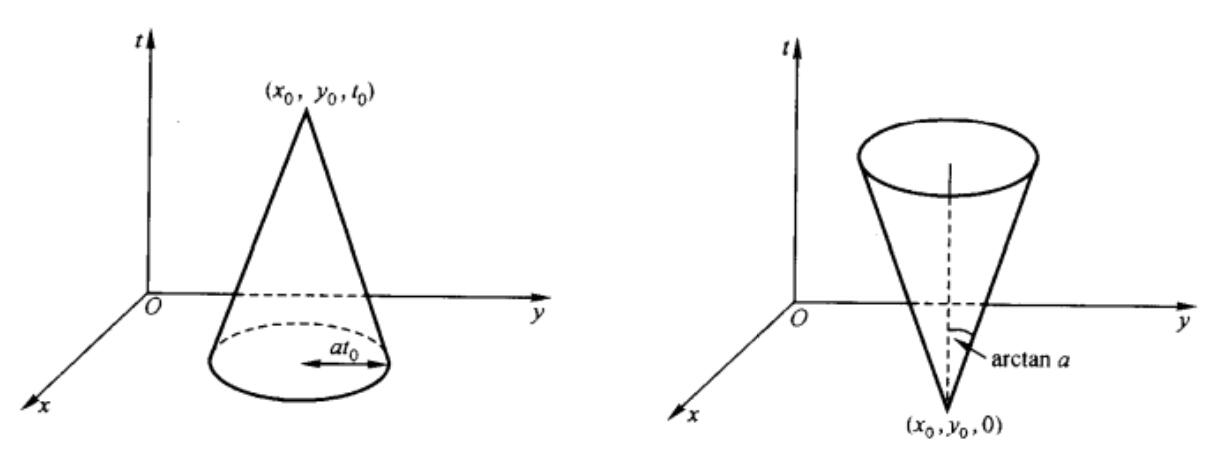
\includegraphics[width=0.5\textwidth]{figure/domain.jpg}
	\caption{决定区域和影响区域 \label{fig:scatter}}
\end{figure}

\par 对于三维问题, \textbf{依赖区域}是球面 $\left(x-x_{0}\right)^{2}+\left(y-y_{0}\right)^{2}+\left(z-z_{0}\right)^{2}=a^{2} t_{0}^{2}$, \textbf{决定区域}是圆锥体 $\left(x-x_{0}\right)^{2}+\left(y-y_{0}\right)^{2}+\left(z-z_{0}\right)^{2} \leqslant a^{2}\left(t_{0}-t\right)^{2}$, 初始平面上点 $\left(x_{0}, y_{0}, z_{0}, 0\right)$ 的影响区域为锥面 $\left(x-x_{0}\right)^{2}+\left(y-y_{0}\right)^{2}+\left(z-z_{0}\right)^{2}=a^{2} t^{2} \quad(t>0)$, 相应有特征锥 $\left(x-x_{0}\right)^{2}+\left(y-y_{0}\right)^{2}+\left(z-z_{0}\right)^{2}=a^{2}\left(t-t_{0}\right)^{2}$. 
 
\subsubsection{Huygens 原理及波的弥散}

\par 三维情况下有波的前阵面和后阵面称为 \textbf{Huygens原理}或 \textbf{无后效现象}, 而二位情况下扰动的影响范围为整个圆, 只有前阵面没有后阵面, 且扰动随着时间的推移扰动慢慢减弱, 称为波的\textbf{弥散}或称\textbf{有后效现象}, 进一步可以推广到奇数维和偶数维的情形.

\subsubsection{波动方程的衰减}
\par 三维波动方程 $|u(M, t)| \leqslant \frac{1}{4 \pi a^{2} t^{2}} \iint_{S_{u t}^{M} \cap B_{p}^{O}}\left|t \psi\left(M^{\prime}\right)+\varphi\left(M^{\prime}\right)+\nabla \varphi\left(M^{\prime}\right) \cdot \overline{M M^{\prime}}\right| d S_{M}\leqslant C t^{-1}$ , 二维有 $t^{-\frac{1}{2}}$ 的速度趋于零, 一维无衰减.

\subsection{能量不等式及解的唯一性与稳定性}


















\end{document}